\documentclass[fleqn,usenatbib]{mnras}

%%% DEBUG SETTINGS - remove at the end %%%%%%%%%%%%%%%
\usepackage{silence} % silence error warinings
\WarningFilter{caption}{Unsupported document class} % caption doesn't know mnras..
\hbadness = 5000
\vbadness = 10000
% \usepackage{}

% MNRAS is set in Times font. If you don't have this installed (most LaTeX
% installations will be fine) or prefer the old Computer Modern fonts, comment
% out the following line
%\usepackage{newtxtext,newtxmath} % not yet supported on arxiv and uni computer
%\usepackage{txfonts}

% Depending on your LaTeX fonts installation, you might get better results with one of these:
%\usepackage{mathptmx}
%\usepackage{txfonts}

% Use vector fonts, so it zooms properly in on-screen viewing software
% Don't change these lines unless you know what you are doing
\usepackage[T1]{fontenc} % make sure font is supported
% \usepackage{ae,aecompl} %obsolete when using modern fonts
\usepackage[final]{microtype} % make sure font is supported
% and a suitable font
\usepackage{lmodern} % use a modern font with T1 support
%\usepackage{cm-super} % use a modern font with T1 support


%%%%% AUTHORS - PLACE YOUR OWN PACKAGES HERE %%%%%

% Only include extra packages if you really need them. Common packages are:
%\usepackage[dvipdfmx]{graphicx}	% Including figure files
\usepackage{graphicx} % Including figure files
%\usepackage[skip=0pt]{subcaption}
\usepackage{amsmath}	% Advanced maths commands
\usepackage{amssymb}	% Extra maths symbols
\usepackage{pifont}	% Extra maths symbols
%\usepackage{bmpsize}  % PS still needs this for correct bounding boxes?


% TODO stuff, comment out for final submit
\usepackage{todonotes} % as long as we are editing...
%\usepackage{showframe} % for debug
%\overfullrule=5pt      % show overfull boxes

% I disabled hyperlink in the cls und included it here because of bugs
\usepackage{hyperref}   % Hyperlinks
\hypersetup{colorlinks=true,linkcolor=blue,citecolor=blue,filecolor=blue,urlcolor=blue}

\edef\smallwidth{0.4\linewidth}

\newcommand{\inclfig}[2]{
  \centering
	\includegraphics[width=\smallwidth]{spaghetti/#2_input}%
	\includegraphics[width=\smallwidth]{spaghetti/#2_img3_ipol}
	\includegraphics[width=\smallwidth]{spaghetti/#2_img1}%
	\includegraphics[width=\smallwidth]{spaghetti/#2_img2}
	\includegraphics[width=\smallwidth]{img/M_encl/#2_M_encl}%
	\includegraphics[width=\smallwidth]{masses/#1_#2_mstel_vs_mtot}
}

\newcommand{\inclfign}[2]{
  \centering
	\includegraphics[width=\smallwidth]{spaghetti/#2_input}%
	\includegraphics[width=\smallwidth]{img/nsynth/#2_nsynth}
	\includegraphics[width=\smallwidth]{spaghetti/#2_img1}%
	\includegraphics[width=\smallwidth]{spaghetti/#2_img2}
	\includegraphics[width=\smallwidth]{img/M_encl/#2_M_encl}%
	\includegraphics[width=\smallwidth]{masses/#1_#2_mstel_vs_mtot}
}

\newcommand*{\rot}{\rotatebox{90}}
\newcommand*{\OK}{\ding{51}}
\newcommand*{\NO}{\ding{55}}

\newcommand{\lenstitle}[1]{\noindent\textbf{#1} --}
\newcommand{\params}[3]{(\(\Theta_\text{E}:#1\), $\varepsilon:#2$, $\alpha_\varepsilon:#3$ )}

\newcommand{\asw}[1]{ASW000#1}
\newcommand{\sw}[1]{SW~#1}
\newcommand{\model}[1]{SL model~#1}

\newcommand{\figref}[1]{\ref{fig:#1}}

\newcommand{\Mstel}{M_{\rm stel}}
\newcommand{\Mhalo}{M_{\rm h}}
\newcommand{\haloindex}{\mathcal{H}}

\title[Short title, max. 45 characters]{Model of lens candidates from
  Space Warps CFHTLS}

% The list of authors, and the short list which is used in the headers.
% If you need two or more lines of authors, add an extra line using \newauthor
\author[R. K\"ung et al.]{
Rafael K\"ung,$^{1}$\thanks{E-mail: rafael.kueng@uzh.ch}
Prasenjit Saha,$^{1}$
Lucy Oswald$^{3}$
%and Fourth Author$^{4}$
\\
% List of institutions
$^{1}$Physik Institut, University of Zurich, Winterthurerstrasse XXX, Zurich 8057, Switzerland\\
$^{2}$Department, Institution, Street Address, City Postal Code, Country\\
$^{3}$Another Department, Different Institution, Street Address, City Postal Code, Country
%$^{4}$Another Department, Different Institution, Street Address, City Postal Code, Country
}

% These dates will be filled out by the publisher
% \date{Accepted XXX. Received YYY; in original form ZZZ}

% Enter the current year, for the copyright statements etc.
\pubyear{2016}

% Don't change these lines
\begin{document}
\label{firstpage}
\pagerange{\pageref{firstpage}--\pageref{lastpage}}
\maketitle

\begin{abstract}
We report modelling follow-up of recently-discovered
gravitational-lens candidates in the CFHT Legacy Survey.  Lens
modelling was done by a small group of specially-interested volunteers
from the Space~Warps citizen-science community who originally found
the candidate lenses.  Models are categorised according to seven
qualitative and quantitive points.  Also included are some
improvements to the modelling software used (SpaghettiLens),
and discussion of strategies for scaling to future surveys
with more and frequent discoveries.

The candidates successfully modelled are all galaxies, with inferred
lensing masses ranging from $\sim10^{11}M_\odot$ to $>10^{13}M_\odot$.
Stellar masses have also been estimated, using photometry from the
CFHTLS pipeline and stellar-population models.  A trend well-known
in nearby galaxies, that star-formation efficiency is maximal for
total masses of $\approx10^{12}M_\odot$ and reduces for both lower and
higher masses, is discernable also in these much more distant
galaxies.
\end{abstract}

\begin{keywords}
gravitational lensing: strong -- keyword2
\end{keywords}

\section{Introduction}

Light deflection at the rim of the Sun is famously $1.75''$.  The
deflection angle can also be expressed in terms of the escape velocity
$2v_{\rm esc}^2/c^2$, with $v_{\rm esc}$ at the solar surface being
$\simeq620\rm\,km/s$.  The Galactic escape velocity at the Sun's
location is similar: $\approx500\rm\,km/s$, typical of massive
galaxies.  Thus, the outer regions of massive galaxies have lensing
deflections comparable to that at the rim of the Sun.  Yet these
quantitatively similar deflections have qualitatively different
consequences.  Light deflection by the Sun must be accounted for in
modern astrometry \citep[see e.g.,][]{2015CQGra..32p5008C} but is not
itself a physics probe in the way it was a century ago.  With distant
galaxies, however, light bending by $\sim1''$ introduces two new
phenomena.  First, for galaxies distant enough that their apparent
size is comparable to the bending angle, light deflection can cause
multiple images of background sources, or strong lensing.  Second, the
gravitational field is dominated by dark matter, hence strong lensing
becomes a probe of dark matter in galaxies.

With no unambiguous dark-matter particle detections so far, dark
matter has studied only through its indirect consequences on galactic
and larger scales.  In most work, dark matter is taken to be a
collisionless non-relativistic fluid (cold dark matter or CDM); in
recent years, the simulation by \cite{2005Natur.435..629S} has been
particularly influential in studying the formation of CDM structures.
Other scenarios have also been considered, such as a cold condensing
boson fluid \citep{2016ApJ...818...89S}.  There is a general
consensus, however, that the origins of galaxy lie in the
gravitational collapse, fragmentation, and mergers of dark-matter
clumps, into which fell gas, cooling through radiative processes to
form dense clouds and eventually stars.  There is, however, much
debate about the details, of which \cite{2012RAA....12..917S} provide
a nice summary.

Strong-lensing galaxies are a useful source of information on the
mutual dynamics and dark matter and gas in galaxies.  The topic has
been explored in several studies
\citep{2009ApJ...703L..51K,2011ApJ...740...97L,2012MNRAS.424..104L,
  2016MNRAS.459.3677L,2016MNRAS.456..870B} but it is desirable to
enlarge the samples from tens of lensing galaxies to thousands.  Doing
so requires finding more lenses, of course, but also modelling their
masses.

Recent searches through the CFHTLS \citep{2012SPIE.8448E..0MC} using
arc-finders
\citep{2012ApJ...749...38M,2014A&A...567A.111M,2014ApJ...785..144G} by
machine learning \citep{2016arXiv160504309P} and by visual inspection
by a citizen-science volunteers
\citep[Space~Warps][]{2016MNRAS.455.1191M} have between them
discovered an average of four lenses per square degree.  So one can be
optimistic about finding many thousands of lenses in the next
generation of wide-field surveys.  The expected flood of new lens
discoveries will need a similarly huge modelling modelling effort to
reconstruct their mass distributions.  To prepare for the challenge of
massive-sample lens modelling, \cite{2015MNRAS.447.2170K} developed a
new modelling strategy, implemented as the SpaghettiLens system.  The
idea is to collaborate with experienced members of the citizen-science
community, who have already participated in lens discovery through
Space~Warps, as well as several other projects involving astronomical
data.  In this paper, we present SpaghettiLens models of
lens-candidates discovered through Space~Warps.

Section~\ref{sec:spl} summarises the SpaghettiLens system and
discusses its ongoing development. A SpaghettiLens model consists of a
statistical ensemble of free-form maps of the sky-projected mass
distribution responsible for lensing.  Each lens candidates in
practice gets modelled several times in a collaborative refinement
process\footnote{See ``Collaborative gravitational lens
  modelling\dots'' in {\tt http://letters.zooniverse.org} especially
  the model tree.}  In this paper we report the most recent model for
each lens, as representing a consensus among modellers, as to the best
that could be achieved with the available data and software.
Photometric lens redshifts are used; source redshifts are set to
$z=2$.  The models can, however, be trivially rescaled to use better
redshift values, as and when they become available.
\cite{2015MNRAS.447.2170K} tested the system on simulated lenses and
identified some areas for improvement.  The first two of those are
taken up in Section~\ref{sec:spl}, along with a further idea. In
\S~\ref{subsec:sourcefit} we introduce fitting of the brightness
profiles of the source.  This feature has not yet been included in
SpaghettiLens, but has been carried out in post-processing for a few
especially interesting candidates.  In \S~\ref{subsec:hires} we show
that making mass maps fine-grained in the central region relieves a
tendency in the earlier work for mass to be too shallow. Then in
\S~\ref{subsec:parameter} we consider the possibility of fitting a
parametric lens model to the model ensemble; so far we have only been
successful at extracting an Einstein radius.

Section~\ref{sec:stellar-mass} explains how we compare the lensing
mass with the mass in stars in the lensing galaxy.  We estimate the
stellar mass by comparing galaxy magnitudes from the CFHTLS pipeline
with the well-known stellar-population models of
\cite{2003MNRAS.344.1000B}.  We then extrapolate the stellar masses to
a halo mass using the abundance-matching prescription of
\cite{2010ApJ...710..903M}.  Naturally, the lensing mass must be more
than the stellar mass but no more than the total halo mass.  We then
introduce what we call a halo index $\haloindex$ which gives an idea
of how the lensing mass compares with these two bounds.

Section~\ref{sec:examples} discusses ten of the systems, including six
systems we found to be particularly interesting.  The online
supplement gives results for all the modelled systems.

In Section~\ref{sec:summary} and Table~\ref{tab:models} we display a
concise characterisation of each modelled system, according to the
image morphology and how clear or indistinct it is, whether the mass
map and synthetic lensed image appear to be plausible, and how the
model mass compares with the estimated stellar and full-halo masses.

\section{Lens Modelling}\label{sec:spl}

SpaghettiLens is an example of a medium-sized collaboration spawned by
a large citizen-science project (in this case Space~Warps).  While
collaboration with volunteers is essential to both, the form of
collaboration is very different.  In Space~Warps, volunteers in a
crowd of $\gtrsim10^4$ make independent contributions.  Each person is
presented with a random selection of survey-patches and invited to (in
effect) vote on each.  The system estimates each volunteer's skill
level according to test-patches interspersed with the real data, and
weights their votes accordingly \citep{2016MNRAS.455.1171M}.  There is
an active forum for volunteers, but since everyone is seeing different
data samples with minimal overlap, the forum has little if any
influence on votes.  With SpaghettiLens, on the other hand, there is a
small group of volunteers and their contributions are interdependent.

A modeller's main input to SpaghettiLens is a sketch of arrival-time
contours on a lensed system.  It gives the locations (or best-guess
locations) of images of point-like sources, along with their ordering
in arrival time, and their parities (minumum, saddle-point or
maximum).  Such a sketch, which we call a spaghetti diagram, tends to
resemble the form of lensed arcs, but it also in effect encodes
encodes a proposal for its mass distribution.  A spaghetti diagram is
read by a server-side numerical engine \citep[GLASS, developed
  by][]{2014MNRAS.445.2181C} which then returns a statistical ensemble
of mass maps.  The mass maps are made up of mass tiles and are
free-form, except that they are required to be concentrated around the
identified lens centre.  They are also required to reproduce the given
image locations, parities and time ordering exactly.  Graphical
representations of the mass map and arrival-time surface are returned
to the user for review.  The user can post these results on a forum,
or discard them and try again.  Volunteers can start the modelling
process afresh, or they can take an existing model from the forum and
modify its input spaghetti diagram or its accompanying options, and
thus obtain a revised model.

\subsection{Improved synthetic images}\label{subsec:sourcefit}

The mass maps produced by current implementation of SpaghettiLens are
based on images of point-like features.  No information about extended
images is used, except in so far as they help the user identify images
of point-like features.  The synthetic images offered to users are
rudimentary, based on sources with conical light profiles.

Volunteers often ask about better indicators to identify wether the
modelling resulted in a ``good'' or ``bad'' model.  We developed a
prototype of a better syntetic image than just the rendering of a
conical profile.  It operates on the composite input image.  The user
has to mask the supposed lensed images.  The algorithm then
establishes a grid on the source plane and projects the masked pixels
of the lense plane back to the source plane.  Multiple lens plane
pixels fall onto one source plane pixel and get averaged.  The new
synthetic image then reverses the mapping, coloring each pixel in the
lens plane with the corresponding values of the source plane pixel.

\begin{figure}
  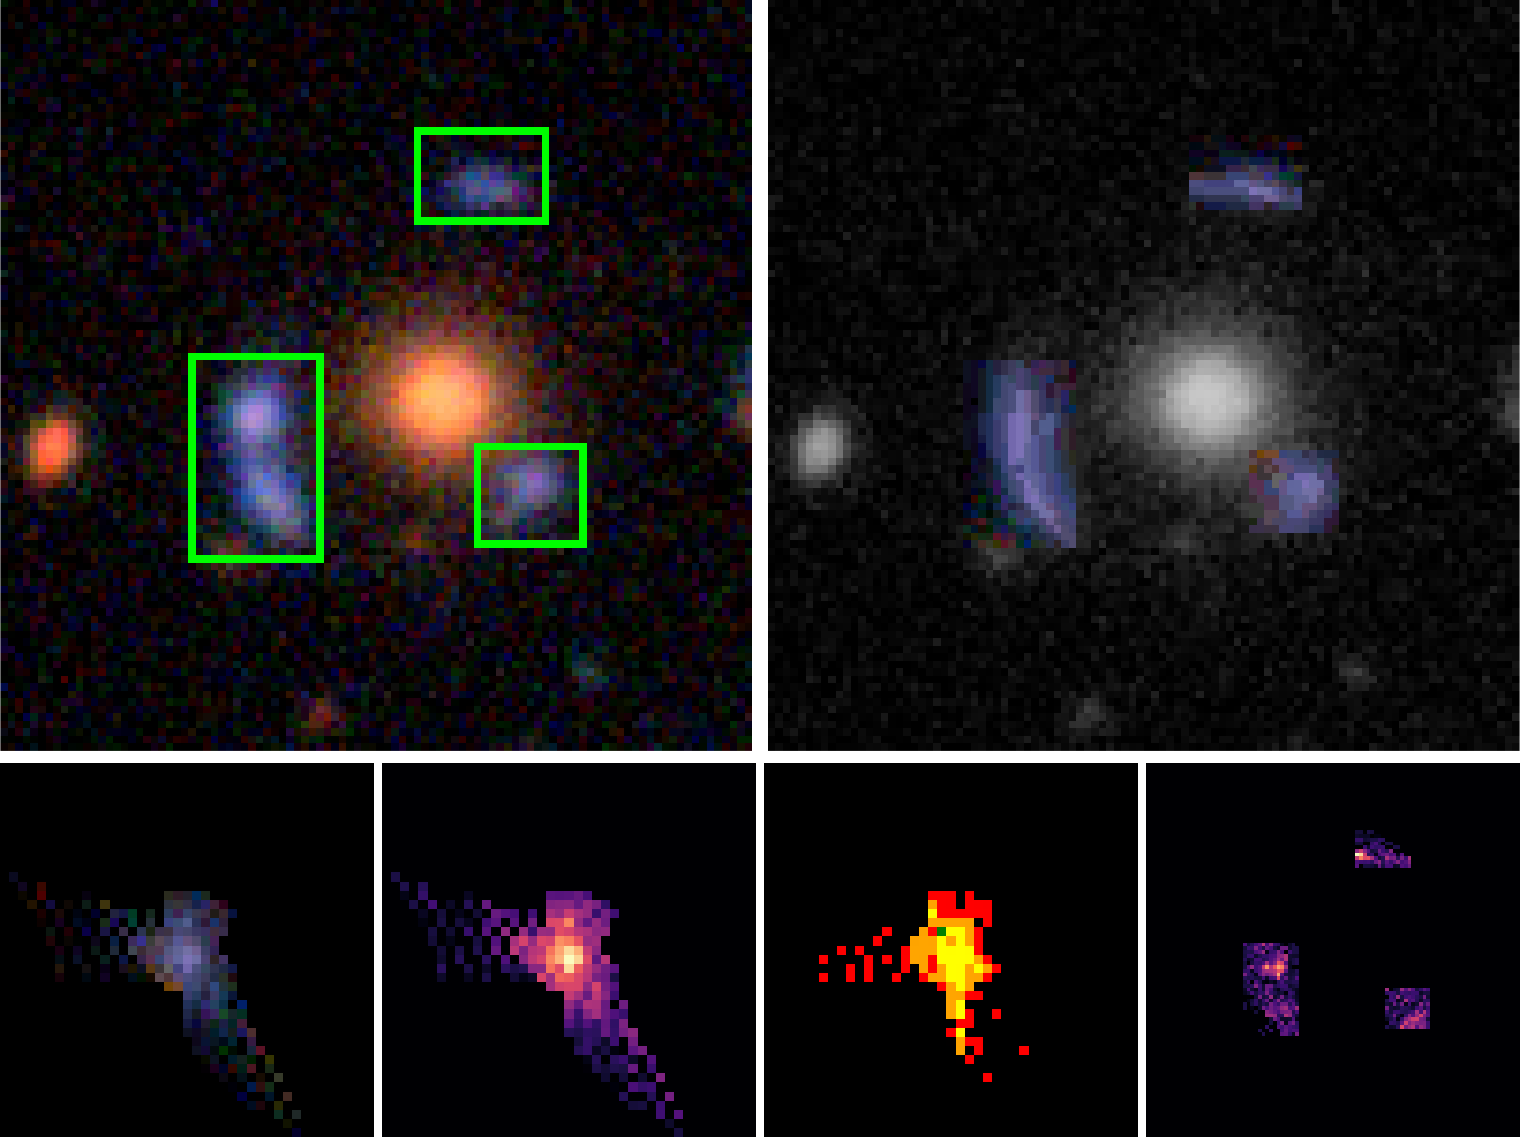
\includegraphics[width=\linewidth]{img/new_synth_img_detailed}
  \caption{Synthetic image with source-profile fitting in SW05
    (J143454.4+522850). Top-left: original image; top-right: synthetic
    image (coloured arcs) with lensing galaxy and unrelated objects in
    greyscale; bottom from left to right: reconstructed source in
    colour, intensity (greyscale), count of lens plane pixels per
    source plane pixel, residual of original image to synthetic
    image.}
  \label{fig:synthimg}
\end{figure}


\subsection{Sub-sampling of central region}\label{subsec:hires}

In a previous paper \cite{2015MNRAS.447.2170K} we identified the problem of the tendency of the models to be too shallow.
We pinned down the problem to the central region and are confident to have it fixed with enabling sub pixel sampling in the central area.
The software allows for subsampling parameters of radius of pixels $r_\text{subs}$ and amount of subpixels per pixel $n_\text{subs}$.
Figure~\figref{subsampling} shows the results of different settings for $r_\text{subs}$ and $n_\text{subs}$.
We can see that even the computationally least expensive settings of $r_\text{subs}=1$ and $n_\text{subs}=3$ leads to drastically improved profiles.

\begin{figure}
  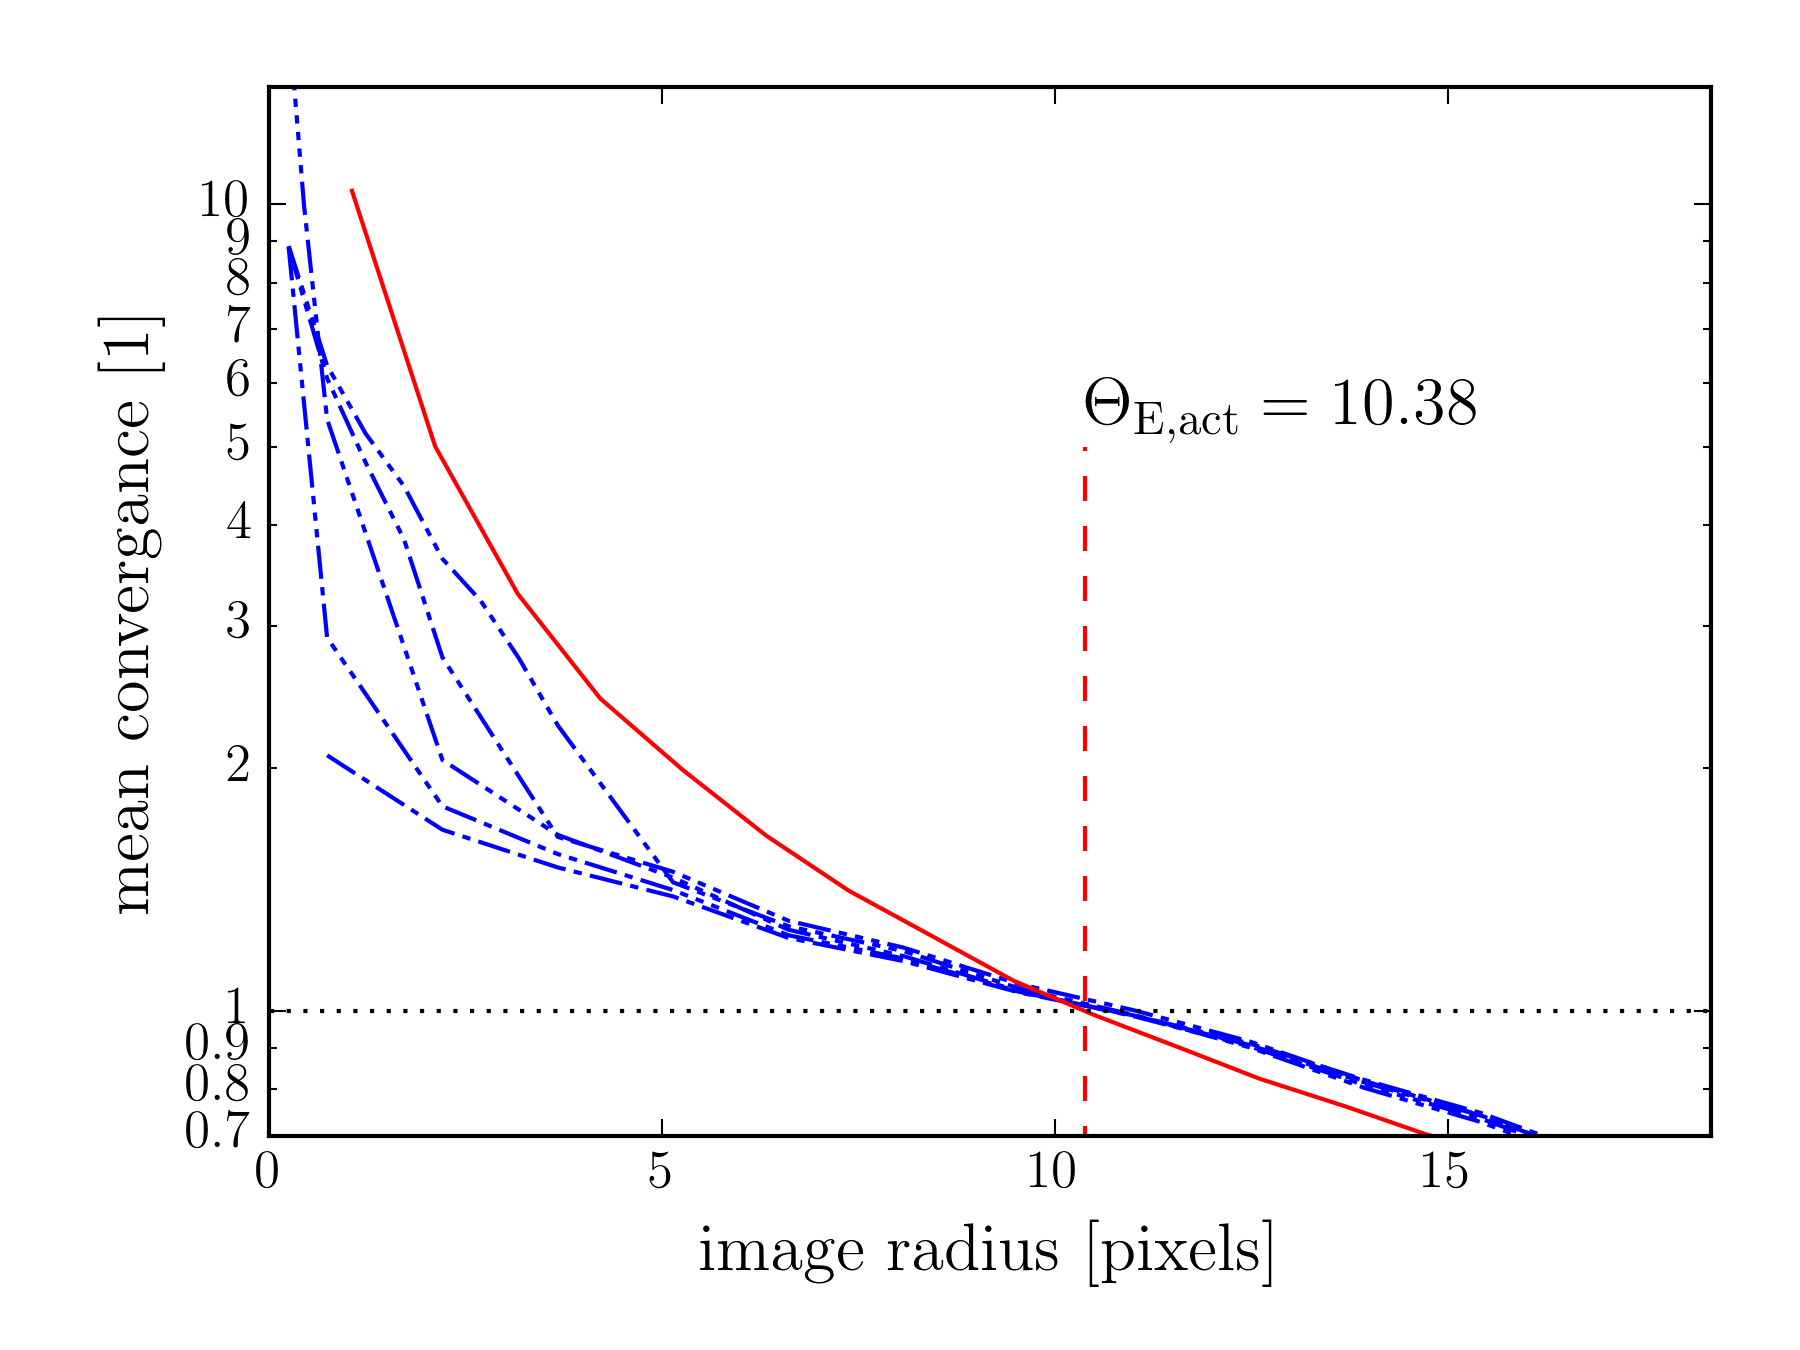
\includegraphics[width=\linewidth]{hires/007022_kappa_encl}
  \caption{
    Circularly averaged mass profile for different subsampling of central region.
    Red line without subsampling, blue lines show subsampling with dash-dot pattern showing the mode.
    $\cdot / \cdot \cdot \cdot$: $r_\text{subs}=1$ inner pixels, each subdivided into $n_\text{subs}=3$ sub pixels.
    $\cdot / \cdot \cdot \cdot \cdot \cdot$: $r_\text{subs}=1$, $n_\text{subs}=5$.
    $\cdot \cdot / \cdot \cdot \cdot $: $r_\text{subs}=2$, $n_\text{subs}=3$.
    $\cdot \cdot \cdot / \cdot \cdot \cdot $: $r_\text{subs}=3$, $n_\text{subs}=3$.
    }
  \label{fig:subsampling}
\end{figure}


\subsection{Parameterisation of pixel models} \label{subsec:parameter}
\todo{}
In order to fit the set of pixelated models to a single parameterised model, a program was written that took a parameterised function and subtracted from it the mean and the principle components of the data, which were calculated using classical Principle Component Analysis.
This created the residuals function.
The number of components defined as principle was varied to test how this affected the output, and it was found that using 5 principle components tended to give a reasonable approximation.
A masking function was added which selected only the data points that fell inside the image of the lens, and the principal components were clipped in order to keep the values inside the region of the ensemble of models.
Any value higher than the clip was set to be the clip value.
This was chosen to be 2.5 as, assuming that the data follows a Gaussian error distribution, almost all the values for the variance should lie between 2 and 3 standard deviations from the mean.
Minimising the residuals function produces the set of parameters that fit the parameterised function to the original pixelated ensemble most closely.
A least squares fit was used to perform this minimisation.
The parameterised model function was obtained from the gravitational potential of an isothermal ellipsoid mass distribution \cite{2001astro.ph..2341K}.
This model is frequently used to describe gravitational lenses as it tends to fit well with observations.
The isothermal ellipsoid model outputs three useful parameters: the radius of the Einstein ring, the ellipticity of the model and the angle of the ellipticity from the vertical, giving the orientation of the galaxy.
By applying this model to simulated lenses for which the values of these parameters were already known, it was possible to gain an estimate of the projected accuracy of the results, before applying the model to the candidate lensing galaxies.

\section{Stellar mass}\label{sec:stellar-mass}

Based on \cite{2003MNRAS.344.1000B} models.\todo{Needs text.}

Following \cite{2010ApJ...710..903M}
\begin{equation}
\begin{aligned}
\frac{\Mstel}{\Mhalo} &= \frac{2C_0}{(\Mhalo/M_1)^{-\beta} +
                                     (\Mhalo/M_1)^\gamma} \\
C_0 &= 0.02820, \quad M_1 = 10^{11.884} M_\odot \\
\beta &= 1.057, \quad \gamma = 0.556.
\end{aligned}
\end{equation}

\begin{equation}
\haloindex = \frac{\ln(M/\Mstel)}{\ln(\Mhalo/\Mstel)}
\end{equation}
which we may call the halo-matching index.
\begin{itemize}
\item $\haloindex < 0$ is unphysical because $M<\Mstel$.
\item $\haloindex = 0$ is when the stellar mass exactly accounts for the
  lensing mass.
\item $0 < \haloindex < 1$ is the typical situation, where the lens
  includes stars and dark matter, but not the full halo.
\item $\haloindex = 1$ means that the lens consists of the entire halo.
\item $\haloindex > 1$ is in tension with abundance-matching, because the
  lensing mass exceeds the expected halo mass.
\end{itemize}


\section{Example systems}\label{sec:examples}

In this section we show modelling results for ten of the lens
candidates.  The first five (see Figures~\figref{SW05}--\figref{SW29})
are the most convincingly modelled systems.  The next three cases
(Figures~\figref{SW42}--\figref{SW19}) are less good but still very
plausible models, and are representative of the majority of the
sample.  The last two are examples where the models were unconvincing
(Figures~\figref{SW36}) or completely failed (\figref{SW57}).

\begin{figure}
  \inclfign{SW05}{ASW0007k4r_AJIBCHQ6EM}
  \caption{Model results for SW05 (J143454.4+522850).  See text in
    Section~\ref{sec:examples} for details.}
  \label{fig:SW05}
\end{figure}

\begin{figure}
  \inclfign{SW28}{ASW0007xrs_JHC3J2HYV7}
  \caption{Model results for SW28 (J143055.9+572431).}
  \label{fig:SW28}
\end{figure}

\begin{figure}
  \inclfign{SW02}{ASW000619d_011489}
  \caption{Model results for SW02 (J140522.2+574333).}
  \label{fig:SW02}
\end{figure}

\begin{figure}
  \inclfign{SW09}{ASW0002asp_5EKMWWVJHL}
  \caption{Model results for SW09 (J020832.1-043315).}
  \label{fig:SW09}
\end{figure}

\begin{figure}
  \inclfign{SW29}{ASW0008qsm_TOFS7JNGEK}
  \caption{Model results for SW29 (J143838.1+572647).}
  \label{fig:SW29}
\end{figure}

\begin{figure}
  \inclfig{SW42}{ASW00096rm_4Q3YCEWGLN}
  \caption{Modelling results for SW42 (J221716.5+015826).}
  \label{fig:SW42}
\end{figure}

\begin{figure}
  \inclfig{SW58}{ASW0007iwp_4XBJWT3COV}
  \caption{Model results for SW58 (J143651.6+530705).}
  \label{fig:SW58}
\end{figure}

\begin{figure}
  \inclfig{SW19}{ASW0001ld7_OS3CYAKLRT}
  \caption{Model results for SW19 (J020642.0-095157).}
  \label{fig:SW19}
\end{figure}


\begin{figure}
  \inclfig{SW36}{ASW000096t_7IPP7LWVOF}
  \caption{Model results for SW36 (J090248.4-010232).}
  \label{fig:SW36}
\end{figure}

\begin{figure}
  \inclfig{SW57}{ASW0008pag_5SXGXQYY6V}
  \caption{Model results for SW57 (J143631.5+571131).}
  \label{fig:SW57}
\end{figure}

Let us first consider Figure~\figref{SW05}, which shows model results
from SW05 (J143454.4+522850).

\begin{enumerate}
\item In the upper row we have first a cutout of the Space~Warps
  image, marked up with a spaghetti diagram.  There are four distinct
  lensed images, and the spaghetti diagram proposes that they are a
  minimum nearest to the lensing galaxy, a close minimum-saddle pair,
  and a minimum further away. In Table~\ref{tab:models} we refer to
  such configurations as `$1+2+1$'.
\item Alongside is a synthetic image produced by modelling.  In it,
  the fitted lensed images are shown in colour, while the lensing
  galaxy and extraneous objects have been reduced to grayscale.
  (Figure~\figref{synthmig} in \S~\ref{subsec:sourcefit} shows a
  synthetic image from another model of the same system.) These two
  panels are qualitative and display no units, and moreover, the
  mutual alignment of the two panels is only approximate.
\item The middle row shows contour maps from the model.  At middle
  left, we have the arrival-time surface.
\item At middle right we have the mass distribution in the usual
  dimensionless form $\kappa$.  Again, these two panels are mainly
  qualitative: both panels are spatially registered and centred on the
  density-peak of the lens, but no scales have been included.
\item The base row supplies spatial and mass scales.  The left panel
  shows the circularly-averaged $\kappa$ of the model ensemble, with
  increasing radius (in arcsec).  The four short vertical lines
  correspond to the minima and saddle points marked in the upper-left
  panel.  The effective Einstein radius is also shown.  As the radius
  scale indicates SW05 is comparatively large lens on the
  sky.\todo{Fix distance factor in $\kappa$.}
\item Lower right shows the total mass in the model against the
  estimated stellar mass, alongside the values for the whole sample.
  The lower-right shaded region is unphysical according to the
  stellar-population models, because it gives $M<\Mstel$. The
  upper-left shaded region is unphysical according to abundance
  matching, because it gives $M>\Mhalo$.  That is to say, the unshaded
  region is $0<\haloindex<1$.
\end{enumerate}

Proceeding to Figure~\figref{SW28}, we have one image close to the
galaxy and an arc further away, which is interpreted as a blend of
three images (a saddle point with two minima on either side).  We call
this a '1+3' configuration.  It is an indication of a mass
distribution elongated along the arc-counterimage direction (along EW
in this case).

In Figures~\figref{SW02}--\figref{SW29} we see three candidates with
an arc close the lensing galaxy and one image further away.  The arc
is interpreted three images (a minimum with two saddle points on
either side).  We call this a '3+1' configuration.  It is an
indication of a mass distribution elongated perpendicular to the
arc-counterimage direction.

Figures~\figref{SW02}--\figref{SW29} (SW05, SW28, SW02, SW09 and SW29)
all correspond to the mass range of massive ellipticals.  SW05 is the
most massive of all the candidates, with a galaxy-group scale mass.

Figure~\figref{SW42} shows SW42.  The image morphology is similar to
SW05 in Figure~\figref{SW05}, but the lens is much smaller on the sky,
and the inferred mass is at the low end of the sample.  (The synthetic
image shown is cruder than for the five previous figures, but that
does not influence the mass models.)  If these preliminary findings
are confirmed by follow-up observations, this could be the most
dark-matter dominated lens known.\todo{Check photometry of this
  candidate.}

Figures~\figref{SW58} and \figref{SW19} appear plausible lens
candidates.  Their morphology is similar to SW28, but the saddle-point
counterimage is not visible.  We consider these lenses plausible but
less convincing.

Figures~\figref{SW36} and \figref{SW57} are cases where modelling
failed.


\section{Summary of models}\label{sec:summary}

Table~\ref{tab:models} 

\begin{enumerate}
\item The image morphology concisely described: D for double, and
  quads in sub-categorised in four ways
  \citep[cf.][]{2003AJ....125.2769S} as LQ for long-axis quads (as in
  Figure~\figref{SW28}), SQ for short-axis quads (as in
  Figure~\figref{SW02}, \figref{SW09}, \figref{SW29}, \figref{SW42}),
  IQ for inclined quads (as in Figure~\figref{SW05}) and CQ for very
  symmetric core quads.
\item Whether the images are unblended.  Distinct unblended images (as
  in Figures~\figref{SW05} and \figref{SW42}) are an advantage in
  modelling, but not essential.
\item Whether all images are discernable.  The topography of an
  arrival-time surface, as encoded by a spaghetti diagram, may require
  more images than are visible.  For example, in Figure~\figref{SW58},
  the modeller has put in a conjectural saddle point near the lensing
  galaxy.
\item Whether the lens is fairly isolated.
\item Whether the arrival-time surface and synthetic image are
  plausible.  In Figure~\figref{SW36} the model implies extra images
  or a long arc, which are not seen.
\item Whether the mass map is reasonable.
\item The halo index $\haloindex$.
\end{enumerate}

\begin{table*}
  \caption{Categorisation of SW models}
  \label{tab:models}
  
\begin{tabular}{c c c | c c | c c c | c c c}
  \hline
  SWID & ASW id & model id
  
    & \rot{$z_\text{lens}$}

    & \rot{\shortstack[l]{image\\morphology}}
    
    & \multicolumn{1}{|l|}{\rot{\shortstack[l]{unblended\\images}}}
    & \rot{\shortstack[l]{all images\\discernible}}
    & \rot{\shortstack[l]{isolated\\ lens}}
    
    & \rot{\shortstack[l]{synthetic image\\ reasonable}}
    & \rot{\shortstack[l]{mass map\\ reasonable}}
    & \rot{\shortstack[l]{total vs stellar\\ mass ratio}}
  \\ \hline
  SW01 & ASW0004dv8 & J022409.5-105807 & 
    & 
    &  &  & 
    &  &  &  \\
    
  SW02 & ASW000619d & J140522.2+574333 & 0.7
    & LQ
    & \NO & \OK & \NO
    & \OK & \OK & 10 \\
    
  SW03 & ASW0006mea & J142603.2+511421 & 
    & 
    &  &  & 
    &  &  &  \\
    
  SW04 & ASW0009cjs & J142934.2+562541 & 0.5
    & CQ
    & \OK & \NO & \NO
    & \NO & \OK & 74 \\
    
  SW05 & ASW0007k4r & J143454.4+522850 & 0.6
    & IQ
    & \OK & \OK & \OK
    & \OK & \OK & 1.0e+02 \\
    
  SW06 & ASW0008swn & J143627.9+563832 & 0.5
    & LQ
    & \NO & \OK & \OK
    & \OK & \NO & 7 \\
    
  SW07 & ASW0007e08 & J220256.8+023432 & 
    & 
    &  &  & 
    &  &  &  \\
    
  SW08 & ASW00099ed & J020648.0-065639 & 0.8
    & D
    & \OK & \OK & \NO
    & \OK & \OK & 7 \\
    
  SW09 & ASW0002asp & J020832.1-043315 & 1.0
    & SQ
    & \NO & \OK & \OK
    & \OK & \OK & 9 \\
    
  SW10 & ASW0002bmc & J020848.2-042427 & 0.8
    & D
    & \OK & \NO & \OK
    & \NO & \NO & 3 \\
    
  SW11 & ASW0002qtn & J020849.8-050429 & 0.8
    & LQ
    & \NO & \OK & \NO
    & \OK & \OK & 3 \\
    
  SW12 & ASW0003wsu & J022406.1-062846 & 0.4
    & D
    & \OK & \OK & \NO
    & \OK & \OK & 4 \\
    
  SW13 & ASW00047ae & J022805.6-051733 & 0.4
    & LQ
    & \NO & \NO & \NO
    & \NO & \NO & 7 \\
    
  SW14 & ASW0004xjk & J023123.2-082535 & 
    & 
    &  &  & 
    &  &  &  \\
    
  SW15 & ASW0004nan & J084841.0-045237 & 0.3
    & LQ
    & \NO & \OK & \NO
    & \OK & \OK & 8 \\
    
  SW16 & ASW0009bp2 & J140030.2+574437 & 0.4
    & D
    & \NO & \NO & \OK
    & \NO & \OK & 5 \\
    
  SW17 & ASW0005rnb & J140622.9+520942 & 0.7
    & D
    & \OK & \NO & \NO
    & \NO & \OK & 6 \\
    
  SW18 & ASW0007hu2 & J143658.1+533807 & 0.7
    & D
    & \OK & \NO & \OK
    & \NO & \NO & 4 \\
    
  SW19 & ASW0001ld7 & J020642.0-095157 & 0.2
    & IQ
    & \NO & \OK & \NO
    & \NO & \OK & 34 \\
    
  SW20 & ASW0002dx7 & J021221.1-105251 & 0.3
    & IQ
    & \OK & \OK & \OK
    & \NO & \OK & 6 \\
    
  SW21 & ASW0004m3x & J022533.3-053204 & 0.5
    & D
    & \OK & \NO & \NO
    & \NO & \OK & 2 \\
    
  SW22 & ASW0009ab8 & J022716.4-105602 & 0.4
    & D
    &  & \NO & \NO
    & \NO & \OK & 2 \\
    
  SW23 & ASW0003r61 & J023008.6-054038 & 0.6
    & ???
    & ? & ? & ?
    & ? & ? & 23 \\
    
  SW24 & ASW00050sk & J023315.2-042243 & 0.7
    & LQ
    & \NO & \OK & \NO
    & \OK & \OK & 2 \\
    
  SW25 & ASW00007mq & J090308.2-043252 & 
    & 
    &  &  & 
    &  &  &  \\
    
  SW26 & ASW0005ma2 & J135755.8+571722 & 0.8
    & D
    & \OK & \NO & \OK
    & \NO & \NO & 9 \\
    
  SW27 & ASW0006jh5 & J141432.9+534004 & 0.7
    & LQ
    & \NO & \NO & \NO
    & \NO & \OK & 10 \\
    
  SW28 & ASW0007xrs & J143055.9+572431 & 0.7
    & LQ
    & \NO & \OK & \NO
    & \OK & \OK & 3 \\
    
  SW29 & ASW0008qsm & J143838.1+572647 & 0.8
    & SQ
    & \NO & \OK & \OK
    & \OK & \OK & 4 \\
    
  SW30 & ASW0002p8y & J021057.9-084450 & 
    & 
    &  &  & 
    &  &  &  \\
    
  SW31 & ASW00021r0 & J021514.6-092440 & 0.7
    & LQ
    & \NO & \OK & \NO
    & \OK & \OK & 24 \\
    
  SW32 & ASW0004iye & J022359.8-083651 & 
    & 
    &  &  & 
    &  &  &  \\
    
  SW33 & ASW0003s0m & J022745.2-062518 & 0.6
    & D
    & \OK & \OK & \NO
    & \NO & \OK & 17 \\
    
  SW34 & ASW00051ld & J023453.5-093032 & 0.5
    & ???
    & ? & ? & ?
    & ? & ? & 10 \\
    
  SW35 & ASW0004wgd & J084833.2-044051 & 0.8
    & LQ
    & \NO & \OK & \NO
    & \OK & \OK & 5 \\
    
  SW36 & ASW000096t & J090248.4-010232 & 0.4
    & D
    & \OK & \OK & \NO
    & \NO & \OK & 9 \\
    
  SW37 & ASW00086xq & J143100.2+564603 & 
    & 
    &  &  & 
    &  &  &  \\
    
  SW38 & ASW0009cp0 & J143353.6+542310 & 0.8
    & LQ
    & \NO & \OK & \OK
    & \OK & \OK & 9 \\
    
  SW39 & ASW0005qiz & J220215.2+012124 & 
    & 
    &  &  & 
    &  &  &  \\
    
  SW40 & ASW0008wmr & J221306.1+014708 & 
    & 
    &  &  & 
    &  &  &  \\
    
  SW41 & ASW0008xbu & J221519.7+005758 & 0.4
    & IQ
    & \OK & \NO & \OK
    & \OK & \OK & 16 \\
    
  SW42 & ASW00096rm & J221716.5+015826 & 0.1
    & IQ
    & \OK & \OK & \NO
    & \OK & \NO & 5.0e+02 \\
    
  SW43 & ASW0001c3j & J020810.7-040220 & 1.0
    & IQ
    & \NO & \NO & \NO
    & \NO & \OK & 6 \\
    
  SW44 & ASW0002k40 & J021021.5-093415 & 0.4
    & ???
    & ? & ? & ?
    & ? & ? & 34 \\
    
  SW45 & ASW00024id & J021225.2-085211 & 0.8
    & R
    & \NO & \OK & \OK
    & \NO & \OK & 8 \\
    
  SW46 & ASW00024q6 & J021317.6-084819 & 0.5
    & D
    & \OK & \OK & \NO
    & \OK & \OK & 6 \\
    
  SW47 & ASW0003r6c & J022843.0-063316 & 0.5
    & D
    & \OK & \NO & \OK
    & \NO & \OK & 26 \\
    
  SW48 & ASW0000g95 & J090219.0-053923 & 
    & 
    &  &  & 
    &  &  &  \\
    
  SW49 & ASW00007ls & J090319.4-040146 & 
    & 
    &  &  & 
    &  &  &  \\
    
  SW50 & ASW00008a0 & J090333.2-005829 & 
    & 
    &  &  & 
    &  &  &  \\
    
  SW51 & ASW0006e0o & J135724.8+561614 & 
    & 
    &  &  & 
    &  &  &  \\
    
  SW52 & ASW0006a07 & J140027.9+541028 & 
    & 
    &  &  & 
    &  &  &  \\
    
  SW53 & ASW00070vl & J141518.9+513915 & 0.4
    & D
    & \OK & \NO & \OK
    & \NO & \OK & 15 \\
    
  SW54 & ASW0007sez & J142620.8+561356 & 0.5
    & R
    & \NO & \OK & \NO
    & \OK & \OK & 16 \\
    
  SW55 & ASW0007t5y & J142652.8+560001 & 
    & 
    &  &  & 
    &  &  &  \\
    
  SW56 & ASW0007pga & J142843.5+543713 & 0.4
    & D
    & \OK & \NO & \OK
    & \NO & \NO & 18 \\
    
  SW57 & ASW0008pag & J143631.5+571131 & 0.7
    & LQ
    & \NO & \OK & \NO
    & \NO & \NO & 64 \\
    
  SW58 & ASW0007iwp & J143651.6+530705 & 0.6
    & SQ
    & \NO & \NO & \OK
    & \OK & \OK & 19 \\
    
  SW59 & ASW00085cp & J143950.6+544606 & 
    & 
    &  &  & 
    &  &  &  \\
    


  \hline

\end{tabular}

\end{table*}

%%%%%%%%%%%%%%%%%%%%%%%%%%%%%%%%%%%%%%%%%%%%%%%%%%
%%%%%%%%%%%%%%%%%%%% REFERENCES %%%%%%%%%%%%%%%%%%
%%%%%%%%%%%%%%%%%%%%%%%%%%%%%%%%%%%%%%%%%%%%%%%%%%

% The best way to enter references is to use BibTeX:
\bibliographystyle{mnras}
\bibliography{bib/bibli} % if your bibtex file is called example.bib


%%%%%%%%%%%%%%%%%%%%%%%%%%%%%%%%%%%%%%%%%%%%%%%%%%
%%%%%%%%%%%%%%%%% APPENDICES %%%%%%%%%%%%%%%%%%%%%
%%%%%%%%%%%%%%%%%%%%%%%%%%%%%%%%%%%%%%%%%%%%%%%%%%

% \appendix

\clearpage

\section{TODO}
\listoftodos

% Don't change these lines
\bsp	% typesetting comment
\label{lastpage}
\end{document}

